% COPIA MARCADA, generada por claude_work/capitulo6_infill_2026_10_07/marcar_cambios.py.
% En azul: texto nuevo o modificado por Claude. No editar este archivo; editar 06_infill.tex.
% !TEX root = ../main.tex

% =====================================================================
% BORRADOR Cap. 6 (07-10-2026), editado sobre capitulos/06_infill.tex.
%   % REVISAR: ...   -> cambio propuesto, para que decidas.
%   % ORIGINAL: ...  -> texto tuyo que se reemplazó.
% Cambios de estructura: \section -> \chapter, \subsection -> \section,
% \subsubsection -> \subsection (clase book). Las etiquetas se conservan.
% =====================================================================

\chapter{Dinámica Radial del Arreglo \textit{Infill} en Simulaciones}
\label{cap:infill}

% REVISAR: "esta sección" -> "este capítulo".
Habiendo validado la fenomenología de la asimetría azimutal en el entorno geométricamente controlado del Anillo Denso, se extendió el análisis a la topología real del arreglo de detectores pero aun utilizando simulaciones. A diferencia del Anillo Denso, el arreglo \textit{Infill} o arreglo regular de $750~m$, permite hacer un estudio sobre las estaciones de superficie y módulos enterrados reales, analizando el comportamiento de la asimetría en un espectro continuo de distancias al eje de la lluvia. Cabe destacar que, para mantener la coherencia con los estudios previos, la mayor parte del análisis desarrollado en este capítulo utiliza exclusivamente la biblioteca de simulaciones de lluvias primarias de protones en el rango de energía de $\log_{10}(E/\mathrm{eV}) \in [17.5, 18.0]$.

% REVISAR: se reemplaza el final del párrafo. La "transición desde un régimen de dominancia cinemática hacia uno de atenuación" no se muestra en el capítulo y no es compatible con el Cap. 3.
% ORIGINAL: "...aislando la física subyacente de la degradación topográfica asociada a los errores sistematicos conocidos propios de la reconstrucción. En este capítulo se aborda cómo la dinámica de la cascada y la resolución del arreglo modulan la asimetría, marcando la transición desde un régimen de dominancia cinemática hacia uno de atenuación longitudinal."
Un objetivo central de esta etapa consistió en caracterizar el impacto de la reconstrucción instrumental sobre la preservación del observable $A_1$. Dado que en el entorno de simulaciones se tiene acceso simultáneo a la geometría verdadera de la lluvia (núcleo y ángulos Monte Carlo) y a su contraparte reconstruida, es posible evaluar el comportamiento del frente de partículas aislando la física subyacente {\color{blue}de la degradación geométrica asociada a los errores sistemáticos propios de la reconstrucción. En este capítulo se aborda cómo la dinámica de la cascada, la reconstrucción y la selección de las estaciones que participan del análisis modulan la asimetría.}

\section{Arreglo \textit{Infill} usando el núcleo y ángulos Monte Carlo}
\label{subsec:infill_mc}

Para comprender la evolución intrínseca de la modulación azimutal, el análisis inicial se ejecutó forzando al \textit{pipeline} de procesamiento a utilizar las coordenadas del núcleo y la dirección de arribo extraídas directamente del nivel Monte Carlo. Esto permite estudiar la respuesta pura de los detectores sin el sesgo del difuminado espacial.

La fuerte dependencia radial y angular de los mecanismos que modulan la densidad de partículas exige una selección topográfica rigurosa. % REVISAR: subsubsec:divergencia ahora apunta a "Respuesta del detector" en el Cap. 3, y la "divergencia cinemática extrema" cerca del núcleo no está establecida. Se deja sólo el argumento de la LDF.
% ORIGINAL: "...la divergencia cinemática extrema descrita en la Sección \ref{subsubsec:divergencia} y el fuerte gradiente de la Función de Distribución Lateral (LDF) inducen fluctuaciones severas en la densidad."
Por un lado, en la región radialmente cercana al centro de impacto ($r < 150$~m), {\color{blue}el fuerte gradiente de la Función de Distribución Lateral (LDF) dentro de cada bin y el bajo número de estaciones inducen fluctuaciones severas en la densidad.} Promediar esta región junto con zonas más lejanas resulta contraproducente, ya que superpone regímenes fenomenológicos contradictorios. Por este motivo, se adoptó un bineado radial dinámico de $\Delta r = 150$~m, aplicando un corte fiducial que excluye dicho \textit{near-core}. 

Simultáneamente, para evitar la mezcla de zonas tempranas y tardías del frente de partículas que diluiría el valor medio de la señal, se particionó la fase azimutal en 12 intervalos ($\Delta\phi = 30^\circ$). Esta necesidad de mantener una alta pureza fenomenológica garantizando al mismo tiempo la robustez estadística en cada bin, definió también la segmentación del ángulo cenital en ventanas de $\Delta \theta = 10^\circ$ (con un intervalo final ampliado para lluvias muy inclinadas, $50^\circ \leq \theta < 65^\circ$). Las grillas completas con los datos junto a los ajustes armónicos y sus respectivos valores de $\chi^2/\text{ndf}$ en este espacio de fases se reportan en el Anexo \ref{anexo:ajustes_infill_mc}.

Al ajustar la densidad de muones registrada por el UMD a la función armónica como se describió en \ref{eq:ajuste_armonico}, se utilizó el estadístico de bondad de ajuste ($\chi^2/\text{ndf} \approx 1$) como métrica fundamental para validar las regiones con asimetría cuantificable. % REVISAR: un chi2/ndf ~ 1 indica compatibilidad con el primer armónico a la precisión disponible; no descarta armónicos superiores.
% ORIGINAL: "Esta convergencia estadística permite demostrar de manera contundente que [...] se describe a la perfección mediante un armónico de primer orden [...], descartando la presencia de términos de orden superior."
{\color{blue}Que este estadístico resulte compatible con la unidad indica que, aislando correctamente las coronas radiales y angulares, la modulación azimutal muónica es compatible con un armónico de primer orden en ciertas regiones bien definidas: con la estadística disponible no se requieren términos de orden superior. Cabe aclarar que las barras de error utilizadas son el error estándar de la media en cada bin, que no contempla la correlación entre los módulos de una misma lluvia; un remuestreo por lluvias da errores en mediana un $10\%$ mayores.}
% REVISAR: el 10% sale de referencia_intento_descartado (bootstrap por lluvia progenitora, mediana 1.10, rango 0.86-1.78). El Cap. 7 usa bootstrap.

En la Figura \ref{fig:a1_vs_r_theta_mc} se sintetizan los resultados de este barrido global, presentando la evolución de la amplitud de asimetría $A_1$ extraída para el UMD en función de la distancia al eje $r$ para las distintas inclinaciones.

\begin{figure}[H]
	\centering
	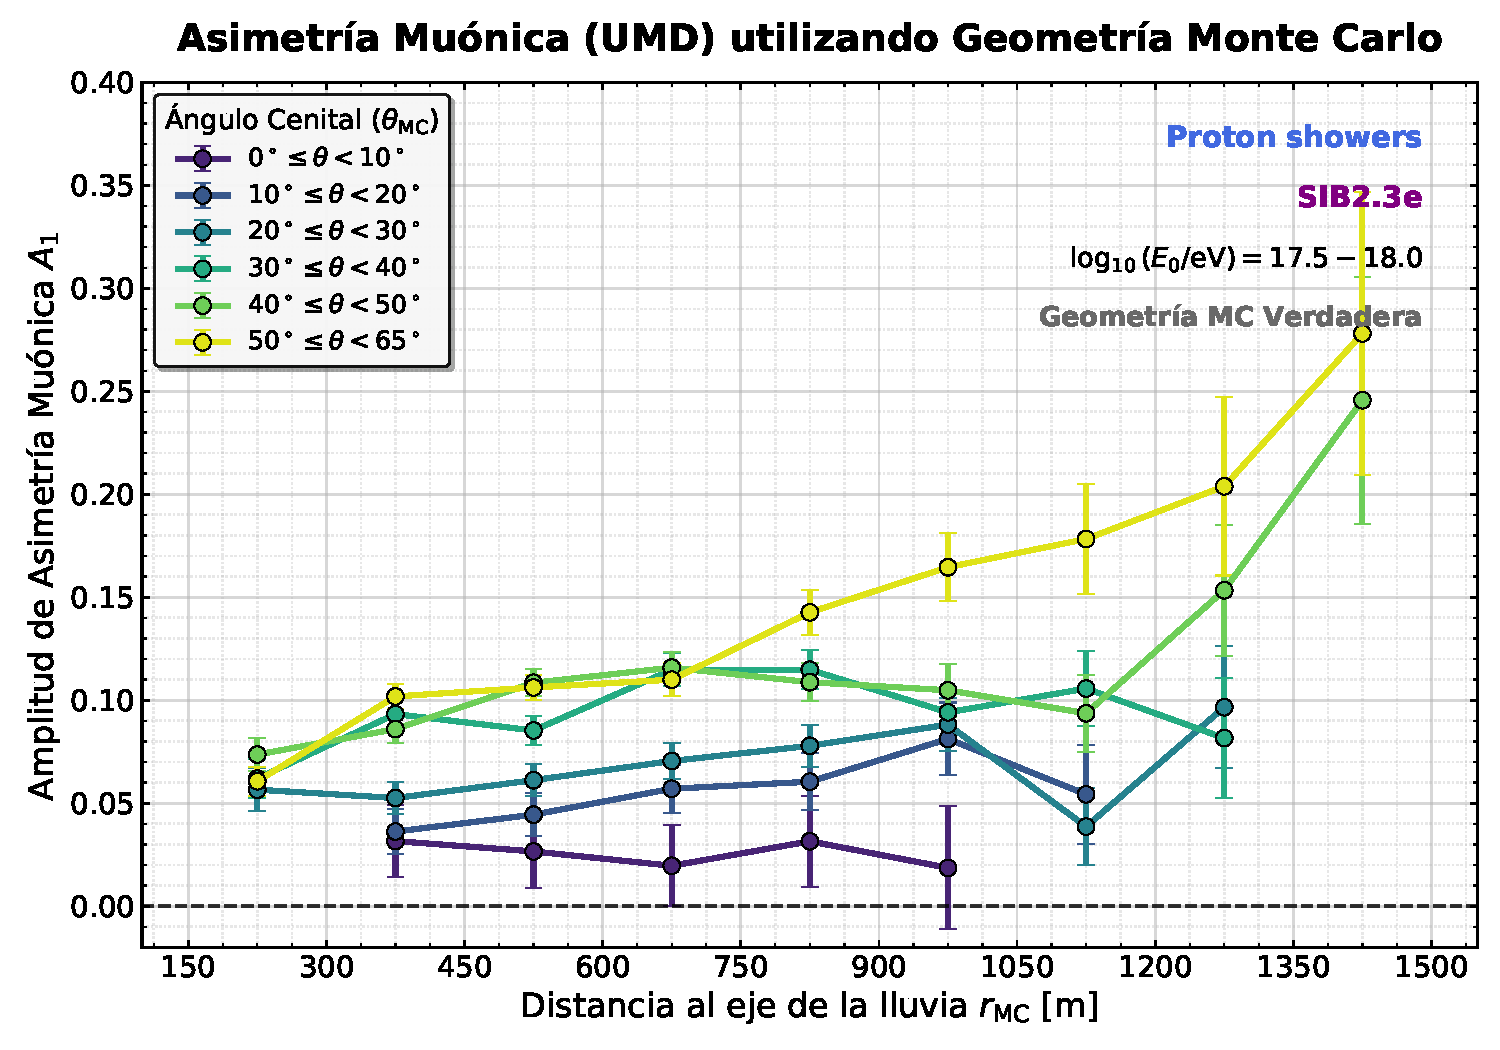
\includegraphics[width=1\textwidth]{capitulos/imagenes_capitulos/cap6/Global_A1_vs_R_Theta_MC.pdf}
	\caption{Evolución de la amplitud de asimetría $A_1$ en función de la distancia al núcleo para distintos rangos de inclinación cenital. El análisis utiliza la geometría verdadera (Monte Carlo) y un bineado radial dinámico ajustado a la viabilidad estadística de cada régimen.}
	\label{fig:a1_vs_r_theta_mc}
\end{figure}

% REVISAR: el "modelo de competencia cinemática-atenuación" ya no existe en el Cap. 3; se remite al modelo de juguete.
% ORIGINAL: "El comportamiento observado confirma las predicciones del modelo de competencia cinemática-atenuación y revela..."
{\color{blue}El comportamiento observado es consistente con lo esperado a partir del modelo de juguete de la Sección~\ref{subsec:toy_models}, una asimetría positiva que crece con la inclinación, y revela los límites de viabilidad estadística del arreglo:}

\begin{itemize}
	\item \textbf{Régimen Vertical ($0^\circ \leq \theta < 10^\circ$):} Como es esperable por simetría geométrica, las lluvias cuasi-verticales no exhiben una dirección temprana o tardía privilegiada frente a la atenuación atmosférica. % REVISAR: no es exactamente nula; el modelo de juguete (Ec. eq:a1_lineal) da un valor pequeño para tan(theta) < 0.1. Verificá los valores en tu figura.
% ORIGINAL: "La modulación azimutal es nula ($A_1 \approx 0$) a lo largo de todo el arreglo."
{\color{blue}La modulación azimutal es pequeña y compatible con cero en todo el rango radial evaluado, como se espera de la Ec.~\ref{eq:a1_lineal} para $\tan\theta \lesssim 0.2$.}
	
	\item \textbf{Régimen Intermedio ($10^\circ \leq \theta < 40^\circ$):} A medida que la lluvia se inclina, la diferencia de recorrido geométrico y la atenuación atmosférica transversal comienzan a romper la simetría. Para inclinaciones moderadas ($10^\circ - 30^\circ$), el observable $A_1$ adquiere valores positivos con un crecimiento de tendencia casi lineal. % REVISAR: lo que cae a ~1100 m es A1, no la densidad.
% ORIGINAL: "...la densidad muónica decae drásticamente lo que se interpreta como causado por fluctuaciones de Poisson severas que parecen resolverse en el siguiente bin radial."
{\color{blue}Sin embargo, a distancias del orden de $\sim 1100$~m la asimetría presenta una caída puntual que se interpreta como una fluctuación estadística, ya que no se mantiene en el siguiente bin radial.} Por su parte, en el siguiente bin angular cenital ($30^\circ - 40^\circ$), aparenta manifestarse un fenómeno de saturación o plateau: la asimetría crece rápidamente pero se estabiliza formando una meseta a partir de los $800$~m.
	
	\item \textbf{Régimen Inclinado ($40^\circ \leq \theta < 65^\circ$):} Para ángulos cenitales grandes, la cantidad de atmósfera atravesada por la cascada se incrementa drásticamente siguiendo la dependencia geométrica de la secante ($X \propto 1/\cos\theta$). % REVISAR: en el Cap. 3 todos los mecanismos escalan con tan(theta) (Ec. eq:a1_lineal); no se muestra que uno sea "dominante absoluto".
% ORIGINAL: "El gradiente longitudinal se vuelve el mecanismo dominante absoluto de la cascada. [...] la enorme diferncia [...] garantiza que la coherencia de la asimetría sea tan robusta que el ajuste sobreviva con alta fidelidad..."
{\color{blue}En consecuencia, crece la diferencia de atmósfera atravesada entre las regiones temprana y tardía.} A diferencia de los regímenes anteriores, el crecimiento de la amplitud $A_1$ es monótono y significativamente mayor, sin presentar saturación. {\color{blue}En estas condiciones, la gran diferencia de densidad de partículas entre las regiones temprana y tardía permite que el ajuste se mantenga estable incluso en la periferia más lejana del arreglo \textit{Infill} ($1350 - 1500$~m).}
\end{itemize}

% REVISAR: la geometría REC no reduce A1 por un factor sino que le resta un término (Sección subsec:infill_rec), así que MC no es una "cota superior". Además, elegir celdas por chi2 o "inspección visual" es un riesgo de look-elsewhere: el código (plots_seccion_6.py) usa r_edges fijados a mano por franja y descarta sólo A1_err > 0.5. Ajustá la frase a tu criterio real.
% ORIGINAL: "Estos resultados demuestran que [...] estableciendo una cota teórica superior para lo que el UMD puede aspirar a medir [...]. La extensión de las curvas fue delimitada aplicando un criterio de selección riguroso: [...] la métrica de bondad de ajuste ($\chi^2/\text{ndf}$) y la inspección fenomenológica visual garantizan la robustez y fidelidad estadística del observable."
{\color{blue}Estos resultados muestran que, en ausencia de incertezas geométricas instrumentales, la asimetría muónica es un observable sensible a la evolución longitudinal de la cascada, y establecen la referencia con la que se comparan, en la Sección~\ref{subsec:infill_rec}, los resultados obtenidos con la geometría reconstruida. Cabe destacar que el dominio radial evaluado no es uniforme, sino que ha sido adaptado a la estadística de cada franja cenital: la extensión de las curvas se limitó a los bines radiales con estadística suficiente para que el ajuste converja, y los ajustes de todas las celdas se reportan en el Anexo~\ref{anexo:ajustes_infill_mc}.}

Es pertinente destacar que, al replicar este mismo análisis sustituyendo la cantidad de muones inyectada ($N_\mu^{\mathrm{MC}}$) por la cantidad reconstruida por el algoritmo del UMD ($N_\mu^{\mathrm{REC}}$), pero manteniendo el núcleo y los ángulos Monte Carlo, la fenomenología global se conserva de forma idéntica. Como se ilustra en la Figura \ref{fig:umd_rec_vs_mc_theta} para  el rango cenital de referencia de $40^\circ \leq \theta < 50^\circ$, la principal consecuencia de introducir la respuesta de la reconstrucción de la cantidad de muones es una atenuación en la magnitud absoluta de la asimetría, sin alterar su forma fundamental ni las transiciones radiales discutidas, {\color{blue}igual que sucedía en la Sección~\ref{subsec:mc_vs_rec}. Se estima que la causa de esta diferencia es la misma que en el Anillo Denso y deviene del funcionamiento de los algoritmos de reconstrucción y su sesgo direccional (Sección~\ref{subsec:bias_direccional}).}

\begin{figure}[H]
	\centering
	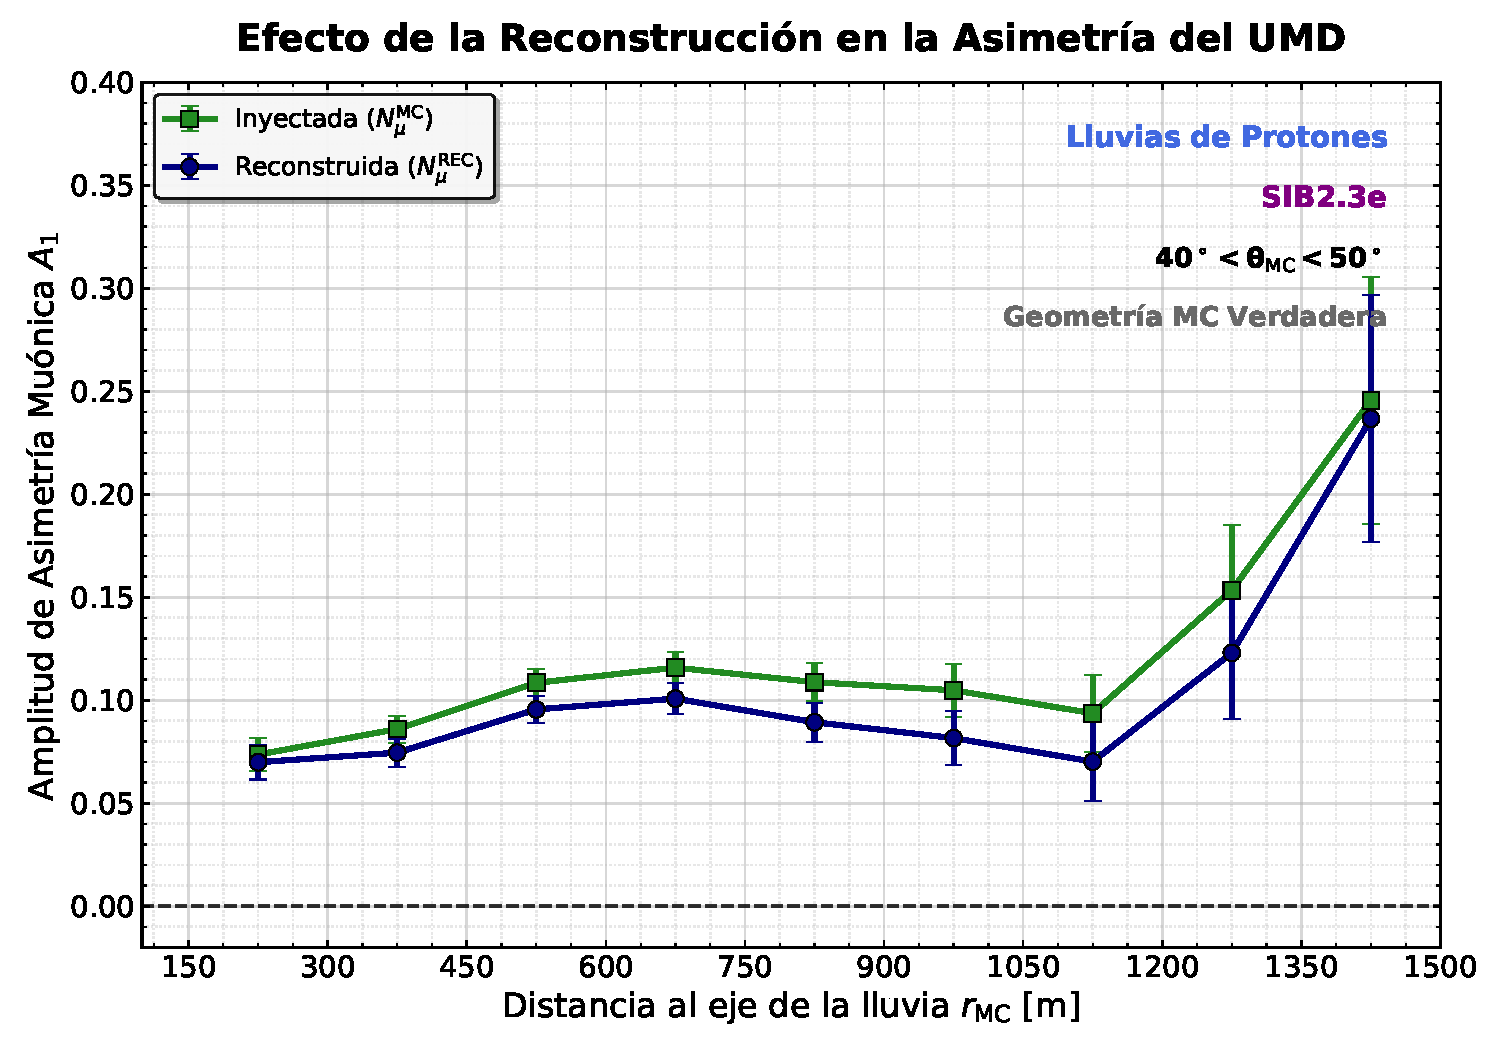
\includegraphics[width=1\textwidth]{capitulos/imagenes_capitulos/cap6/UMD_Asymmetry_MC_vs_REC.pdf}
	\caption{Comparación de la amplitud de asimetría $A_1$ obtenida a partir del número de muones inyectado ($N_\mu^{\mathrm{MC}}$) frente al número de muones reconstruido ($N_\mu^{\mathrm{REC}}$) para el rango cenital de referencia de $40^\circ \leq \theta < 50^\circ$. Ambas se realizan fijando las coordenadas a nivel Monte Carlo. Se observa que la respuesta instrumental del detector introduce una atenuación sistemática en la magnitud de la asimetría, preservando la evolución radial.}
	\label{fig:umd_rec_vs_mc_theta}
\end{figure}

\subsection{Competencia de observables: UMD frente al SD Total}
\label{subsubsec:umd_vs_sd_mc}

Con la fenomenología muónica del UMD caracterizada, el siguiente paso analítico consistió en contrastar este comportamiento frente a la señal total registrada por los tanques Cherenkov en superficie. Resulta importante realizar una distinción fundamental respecto a las variables físicas analizadas: mientras que el detector subterráneo proporciona un conteo directo del número de partículas muónicas incidentes reconstruidas, el SD registra la energía depositada en el volumen de agua, calibrada en unidades VEM, también a partir de la reconstrucción. % REVISAR: además de la señal, también difiere qué estaciones entran en el promedio (Sección subsec:seleccion_estaciones).
% ORIGINAL: "...asegurando que cualquier divergencia observada se deba puramente a la naturaleza de la señal detectada a nivel del suelo."
Para garantizar la validez fenomenológica de este contraste, se mantuvo estrictamente la geometría Monte Carlo, {\color{blue}de modo que las diferencias observadas se deban a la naturaleza de la señal detectada o a la forma en que se seleccionan las estaciones que participan del promedio (Sección~\ref{subsec:seleccion_estaciones}).}

Si analizamos para el bin radial que incluye $\sim 450$~m se puede ver que, análogamente como sucedía para el Anillo Denso, la asimetría detectada por el SD es significativamente mayor a la del UMD. {\color{blue}Además, ambas asimetrías calculadas tienen magnitudes comparables a las encontradas en el Capítulo~\ref{sec:cap_anillo_denso}.} Esto permite ver que los análisis realizados en ambos marcos son comparables y consistentes.

Al extraer la amplitud de asimetría sobre la señal del SD, la curva resultante $A_1(r, \theta)$ expone un comportamiento espacial sistemáticamente distinto al del detector subterráneo. Como se evidencia en la Figura \ref{fig:umd_vs_sd_mc} para un rango cenital de referencia de $30^\circ \leq \theta < 40^\circ$, mientras que el UMD exhibe un crecimiento suave hacia una asimetría positiva a grandes distancias (aun en este rango cenital donde se ve un amesetamiento), el observable del SD presenta una pronunciada inversión fenomenológica. En el régimen donde el gradiente atmosférico debería garantizar una marcada asimetría positiva, la amplitud del SD alcanza un máximo local, comienza a suprimirse y finalmente se invierte, adoptando valores de asimetría fuertemente negativos en la periferia del centro de la lluvia. 

\begin{figure}[H]
	\centering
	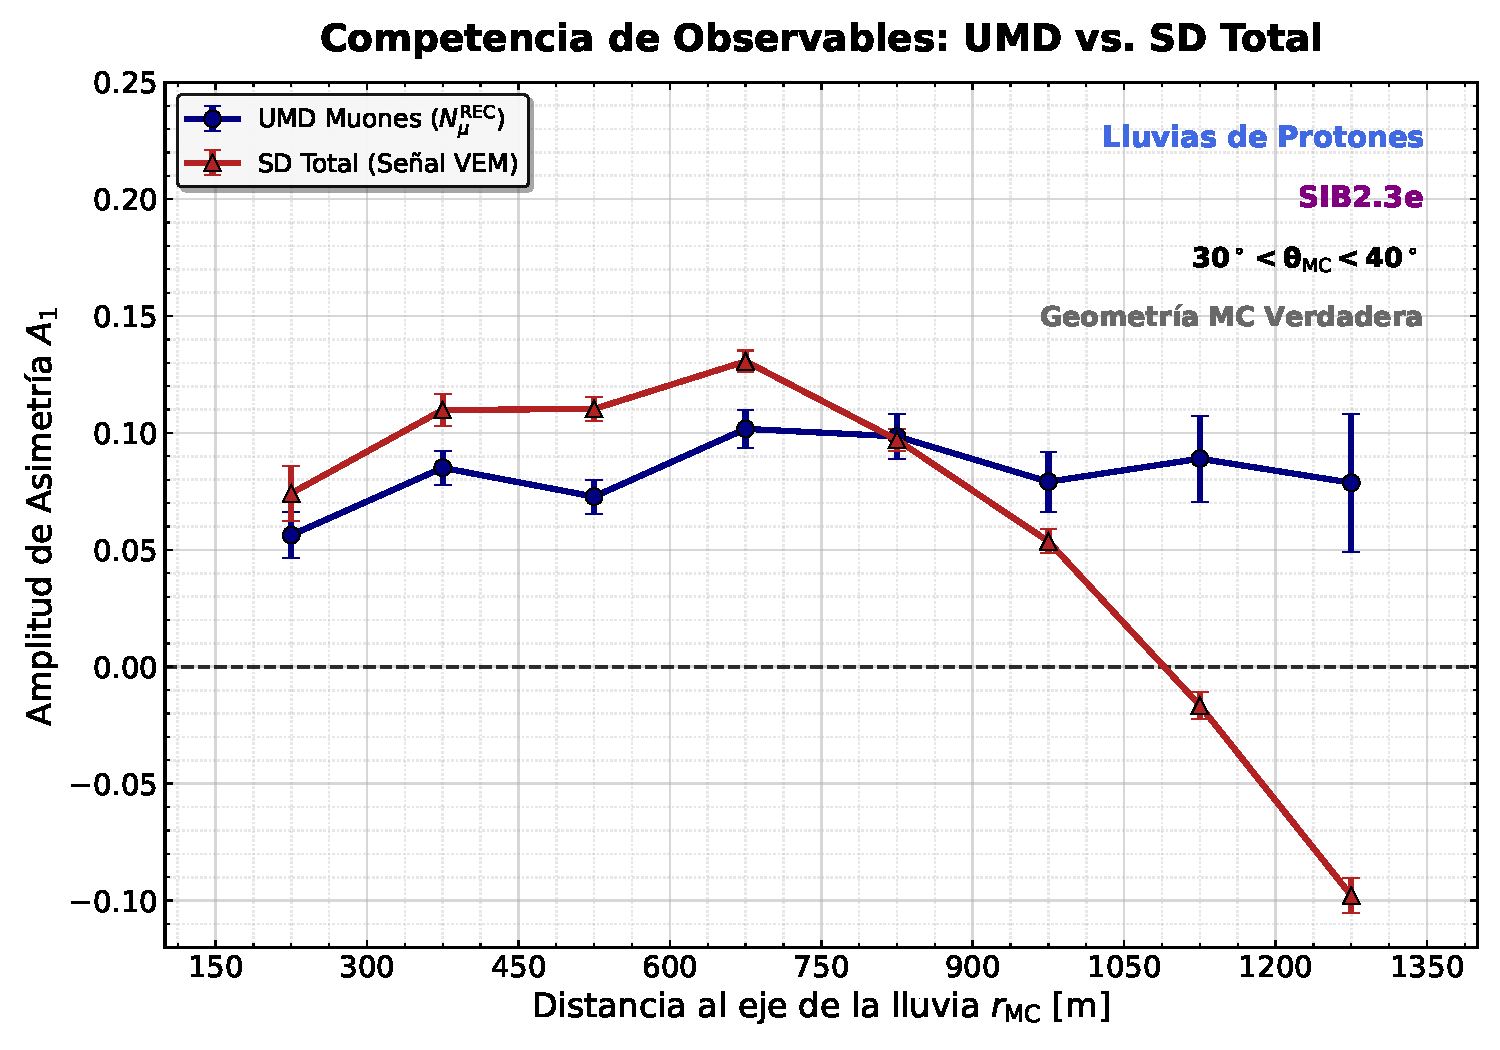
\includegraphics[width=1\textwidth]{capitulos/imagenes_capitulos/cap6/UMD_vs_SD_Total_Asymmetry.pdf}
	% REVISAR: en esta figura el UMD es N_mu^REC (plots_seccion_6.py, celda UMD vs SD); en la del desglose es N_mu^MC. El UMD no crece de forma monótona a 30-40 grados (vos mismo describís la meseta). Las barras son el error estándar de la media.
	% ORIGINAL caption: "...entre la componente muónica pura del UMD y la señal total [...] mientras que el UMD presenta un incremento monótono condicionado por la atenuación, la señal del SD Total exhibe una severa disminucion..."
	\caption{\textcolor{blue}{[caption modificado]} Comparación de la evolución radial de la amplitud de asimetría $A_1$ entre el número de muones reconstruido por el UMD ($N_\mu^{\mathrm{REC}}$) y la señal total registrada por los tanques del SD en superficie, evaluada para el rango cenital de referencia de $30^\circ \leq \theta < 40^\circ$. Ambas curvas fueron extraídas fijando la geometría real de Monte Carlo; las barras de error representan el error estándar de la media. Se evidencia el comportamiento divergente de los observables: mientras que el UMD mantiene una asimetría positiva a todas las distancias, la señal del SD Total exhibe una severa disminución de la asimetría que culmina en una inversión (asimetría negativa) en el \textit{far-core}.}
	\label{fig:umd_vs_sd_mc}
\end{figure}

% REVISAR: el control HasStation (Sección subsec:seleccion_estaciones) muestra que la inversión depende de qué estaciones entran en el promedio; no es una propiedad de la cascada.
% ORIGINAL: "Esta inversión geométrica no es un artefacto de reconstrucción, sino una propiedad física intrínseca de la cascada registrada a nivel del suelo, sugiriendo que el tanque Cherenkov integra poblaciones de partículas con asimetrías diametralmente opuestas."
{\color{blue}Esta inversión aparece aun con la geometría Monte Carlo, por lo que no se debe a errores en el núcleo ni en la dirección reconstruidos. Para identificar su origen se desglosa a continuación la señal del tanque en sus componentes.}

\subsection{Desglose de señales: La inversión de la asimetría muónica}
\label{subsubsec:desglose_sd}

Para entender el origen físico del comportamiento anómalo del Detector de Superficie al compararse con el Subterráneo, se aprovechó la trazabilidad de las simulaciones para desglosar la señal VEM total en sus dos componentes formativas: la componente electromagnética (electrones y fotones) y la componente muónica medida a nivel del suelo. 

Cabe destacar que existe una diferencia sustancial en el tipo de señales que se están contrastando. La señal declarada como SD Total es la combinación energética de ambas componentes, pero es obtenida a través de la reconstrucción instrumental. Esta señal se calibra a partir de las trazas registradas en los fotomultiplicadores utilizando como referencia la medición del Muón Equivalente Vertical (VEM). En cambio, las componentes por separado que se analizan en esta sección representan la cantidad pura de partículas incidentes a nivel del suelo (nivel Monte Carlo). 

Al evaluar la asimetría de manera independiente para cada población, {\color{blue}se observa una competencia radial}, ilustrada en la Figura \ref{fig:desglose_sd_mc}. Por un lado, la componente electromagnética del SD exhibe una asimetría fuertemente positiva en todo el espectro radial. Dado que estas partículas se regeneran y absorben continuamente, su densidad está acoplada casi instantáneamente al perfil de desarrollo longitudinal de la cascada, convirtiéndolas en un trazador puro de la atenuación atmosférica. Se observa también un comportamiento singular: una estabilización (meseta) de la asimetría para todos los bines radiales por encima de los $\sim 600$~m. Si bien este fenómeno ocurre en diversas franjas cenitales, los estadísticos de bondad de ajuste en esta región profunda decrecen, lo que sugiere que la estabilización podría estar ligada a fluctuaciones estadísticas debido a la atenuación de la componente electromagnética a grandes distancias. {\color{blue}Otra posibilidad es la selección de estaciones discutida en la Sección~\ref{subsec:seleccion_estaciones}: a partir de $\sim 900$~m las estaciones tardías retenidas tienen proporcionalmente más partículas electromagnéticas que las tempranas, lo que tiende a reducir la asimetría medida.}
% REVISAR: oración nueva. A 1050-1200 m (30-40 grados) el número medio de e+gamma de las estaciones retenidas respecto de todas es x1.13 en la región temprana y x1.31 en la tardía (claude_work/capitulo6_infill_2026_10_07/referencia_intento_descartado/factores_seleccion_30_40.csv). Es una candidata, no un resultado.

Por otro lado, la asimetría de los muones registrados por el SD exhibe un comportamiento transicional. {\color{blue}Es aquí donde se encuentra la diferencia principal con el UMD}, dado que el SD registra muones superficiales que, en los primeros bines radiales, se comportan de manera análoga al UMD (con una asimetría positiva creciente). Sin embargo, al acercarse a bines de mayor radio ($\sim 600$~m), la fenomenología cambia drásticamente y la magnitud de asimetría comienza a decrecer, invirtiendo su polaridad hacia valores fuertemente negativos en el \textit{far-core}. {\color{blue}Este comportamiento arrastra a la señal total del SD, que a grandes distancias del eje sigue la tendencia de su componente muónica. Luce \textit{et al.} \cite{Luce_ICRC2021} reportan para la componente muónica de la señal del SD una asimetría levemente negativa ($|A_1| \lesssim 0.05$) entre $1500$ y $2000$~m, de menor magnitud y a mayores distancias que la observada aquí.}
% REVISAR: "ya había sido descripto por la Colaboración" no tenía cita. Luce et al. es lo más cercano, pero mide la componente muónica de la SEÑAL del SD (no el conteo), a mayores distancias y con menor magnitud. También se cambió "el mayor hallazgo analítico" por "la diferencia principal con el UMD".
% ORIGINAL: "Este fenómeno condiciona por completo a la señal total del SD, evidenciando que, a grandes distancias del eje, la asimetría del tanque Cherenkov está dominada por la población muónica de superficie. Este fenómeno ya había sido descripto con anterioridad por la Colaboración."

% REVISAR: se eliminan los tres párrafos de la "Población B". Contradicen el Cap. 3 final: el término de Bertou y Billoir (Ec. eq:efecto_geo) es siempre positivo y es la respuesta de un detector plano; no "explota" con valores negativos. El modelo de juguete da A1 > 0 para el UMD y el SD en todos los casos, y sólo los muones con p > p* favorecen la región tardía. Además, subsubsec:divergencia ahora apunta a "Respuesta del detector".
% ORIGINAL (resumen): "El origen físico de esta inversión se explica de manera natural al recuperar la fenomenología desarrollada en la Sección \ref{subsubsec:divergencia}. [...] se inunda abrumadoramente de la denominada Población B: muones de baja energía [...] provocando que el factor $\langle p_r / -p_z \rangle$ explote a grandes distancias radiales con valores negativos. [...] En consecuencia, la inversión observada en el SD Total es el resultado determinista de convolucionar un frente electromagnético asimétrico positivo con este fondo muónico superficial dominado por el efecto geométrico."
{\color{blue}El Capítulo~\ref{sec:fenomenologia} mostró que esta inversión no puede explicarse con la propagación de los muones. La densidad de muones que incide sobre el suelo tiene una asimetría positiva tanto para el UMD como para el SD (Sección~\ref{subsec:toy_models}), el término de Bertou y Billoir (Ec.~\ref{eq:efecto_geo}) es siempre positivo, y la divergencia cinemática sólo favorece a la región tardía para muones de momento mayor que $p^* \simeq 2QD/r$ (Ec.~\ref{eq:p_cruce}), que son escasos a grandes distancias. El origen debe buscarse, entonces, en la forma en que se construye el observable, lo que se analiza en la Sección~\ref{subsec:seleccion_estaciones}.}


\begin{figure}[H]
	\centering
	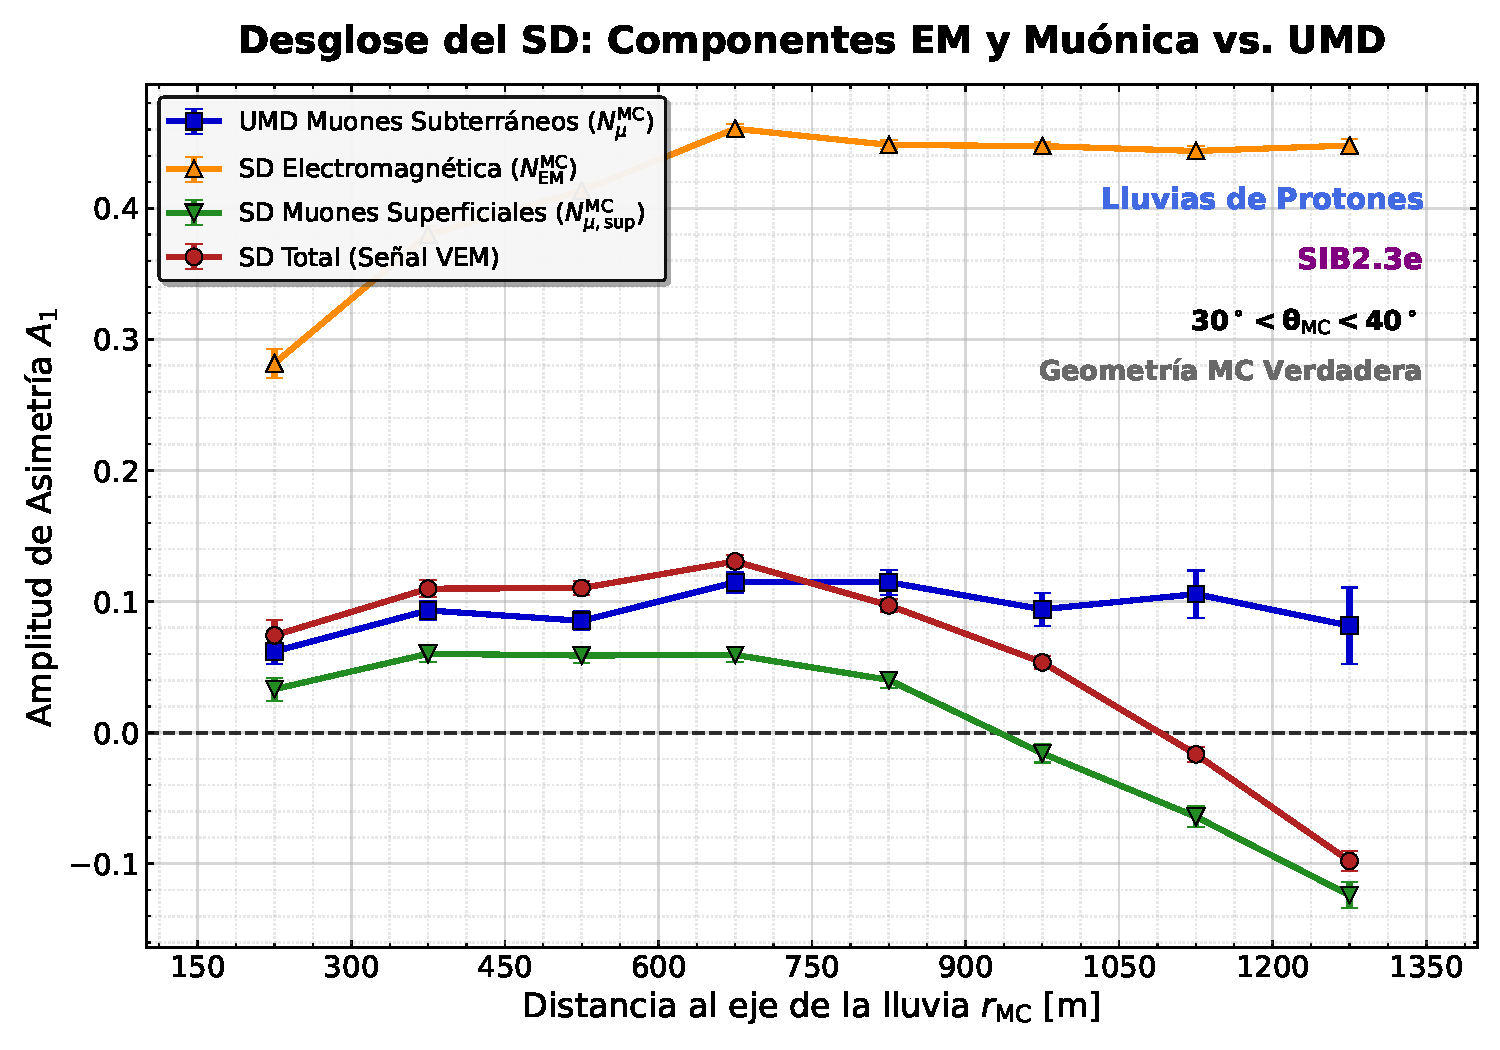
\includegraphics[width=1\textwidth]{capitulos/imagenes_capitulos/cap6/SD_Desglose_Componentes_vs_UMD.pdf}
	% REVISAR: Luce et al. no sostienen la explicación por "dispersión geométrica"; se reemplaza por la selección. En esta figura el UMD es N_mu^MC.
	% ORIGINAL caption: "...los muones superficiales del SD (verde) presentan una asimetría negativa a grandes distancias, producto del efecto de dispersión geométrica por proyección del disco \cite{Luce_ICRC2021}."
	\caption{\textcolor{blue}{[caption modificado]} Desglose de la asimetría azimutal para las componentes inyectadas a nivel del suelo frente al número de muones inyectado en el detector subterráneo ($N_\mu^{\mathrm{MC}}$), para $30^\circ \leq \theta < 40^\circ$ y geometría Monte Carlo. La asimetría electromagnética del SD (naranja) exhibe un comportamiento marcadamente positivo acoplado a la evolución longitudinal. En contraste, los muones del SD (verde) presentan una asimetría negativa a grandes distancias cuando se calcula sobre las estaciones que forman parte del evento reconstruido (Sección~\ref{subsec:seleccion_estaciones}). Las barras de error representan el error estándar de la media.}
	\label{fig:desglose_sd_mc}
\end{figure}

% REVISAR: se reemplazan los tres párrafos sobre el UMD como "filtro cinemático". Contradicen el Cap. 3 final: elevar el umbral hace a A1 MENOS positiva (Sección subsubsec:toy_resultados), y A_geo no se anula para el UMD; es justamente su respuesta de placa (kappa = 1, Sección subsubsec:respuesta_detector). Su lugar lo ocupa la subsección de selección de estaciones, que salió del Cap. 3.
% ORIGINAL (resumen): "La comparación con el UMD valida empíricamente este modelo analítico y demuestra la superioridad instrumental del detector subterráneo. El blindaje pasivo de 2.3 m de tierra actúa como un filtro cinemático estricto [...] ($\lim_{p_z \to \infty} \mathcal{A}_{geo} \to 0$) [...] En conclusión, este desglose poblacional demuestra de manera irrefutable que [...] estableciéndose al UMD como un instrumento fenomenológicamente superior para aislar la asimetría longitudinal."

% REVISAR: subsección nueva. El texto de la Ec. eq:seleccion y el ejemplo de Poisson se adaptaron del Cap. 3 anterior
% (git show fbe13f3:claude_work/capitulo3_unificado_2026_09_30/03_fenomenologia.tex, l. 340-360). El Cap. 3 final (DRAFTS/03, l. 8) todavía promete esta discusión en su introducción: conviene cambiar esa frase para que remita a este capítulo.
\subsection{Selección de estaciones y la inversión del SD}
\label{subsec:seleccion_estaciones}

{\leavevmode\color{blue}Los resultados anteriores no miden la densidad de muones que \textit{incide} sobre el suelo, sino un promedio sobre las estaciones que forman parte del análisis, y una estación sólo forma parte del análisis si la estación del SD disparó y fue incluida en la reconstrucción del evento. Aun cuando el número de muones de cada estación sea exacto, como en el conteo Monte Carlo de las simulaciones, el promedio sobre las estaciones seleccionadas puede diferir del promedio sobre todas.}

{\leavevmode\color{blue}Esto ocurre cuando la probabilidad de que una estación sea seleccionada depende de su propio contenido de muones. Si se denota por $\varepsilon$ la fracción de estaciones seleccionadas en un intervalo de $(r,\phi)$, y por $\varepsilon_N$ la fracción de los muones de ese intervalo que se encuentra en estaciones seleccionadas, el número medio de muones por estación seleccionada es
\begin{equation}
	\langle N_\mu \rangle_{\text{sel}} = \langle N_\mu \rangle_{\text{todas}}\;\frac{\varepsilon_N}{\varepsilon}.
	\label{eq:seleccion}
\end{equation}
Si la selección no depende de los muones, ambas fracciones coinciden y el promedio no cambia. Si las estaciones con más muones tienen más probabilidad de ser seleccionadas, $\varepsilon_N > \varepsilon$ y el promedio seleccionado es mayor que el verdadero. Lo relevante para la asimetría es que este cociente puede ser distinto en la región temprana y en la tardía.}

{\leavevmode\color{blue}Un ejemplo numérico ilustra el efecto. Supóngase que a un radio grande el número medio de muones por estación es $0.6$ en la región temprana y $0.5$ en la tardía, es decir, $A_1 = +0.09$. En la región temprana la componente electromagnética es suficiente para que todas las estaciones disparen, de modo que $\varepsilon = \varepsilon_N = 1$ y el promedio seleccionado es $0.6$. En la tardía, la componente electromagnética está más atenuada, y supóngase que una estación sólo dispara si contiene al menos un muón. Con una distribución de Poisson, sólo el $39\%$ de las estaciones tardías es seleccionado ($\varepsilon=0.39$), pero esas estaciones contienen todos los muones ($\varepsilon_N=1$), y el promedio seleccionado es $0.5/0.39 = 1.27$. La asimetría medida sobre las estaciones seleccionadas es $A_1 = (0.6-1.27)/(0.6+1.27) = -0.36$: el signo se invierte sin que se haya creado ni desplazado ningún muón. Lo que cambió es la población de estaciones sobre la que se calcula el promedio.}

% REVISAR: procedencia de los números de los dos párrafos siguientes: claude_work/revision_asimetrias_sd_umd/02_notebooks/03_sd_vs_umd/ (comparar_sd_umd.py, RESULTADO.md, comparacion_directa.csv) y claude_work/capitulo6_infill_2026_10_07/referencia_intento_descartado/ (factores_seleccion_30_40.csv, retencion_vs_muones_900_1350.csv). La figura sale de la última celda de Scripts/plots_seccion_6.py.
{\leavevmode\color{blue}Para verificar si este mecanismo opera en las simulaciones, se recalculó la asimetría del conteo Monte Carlo de muones del SD para las mismas lluvias de protón ($30^\circ \leq \theta < 40^\circ$), pero sobre todas las estaciones simuladas, sin exigir que formen parte del evento reconstruido. Los errores se estimaron con un \textit{bootstrap} sobre las $960$ lluvias de la muestra, que mantiene juntas las estaciones y los módulos de una misma lluvia. El resultado se presenta en la Figura~\ref{fig:seleccion_estaciones}. Sobre todas las estaciones, la asimetría de los muones del SD es positiva a todas las distancias, entre $+0.03$ y $+0.07$. Al exigir que la estación forme parte del evento, los valores no cambian hasta $\sim 750$~m, donde prácticamente todas las estaciones son seleccionadas, pero luego decrecen hasta $A_1 = -0.124 \pm 0.019$ en $1200$--$1350$~m, frente a $+0.069 \pm 0.016$ sobre todas las estaciones.}

\begin{figure}[H]
	\centering
	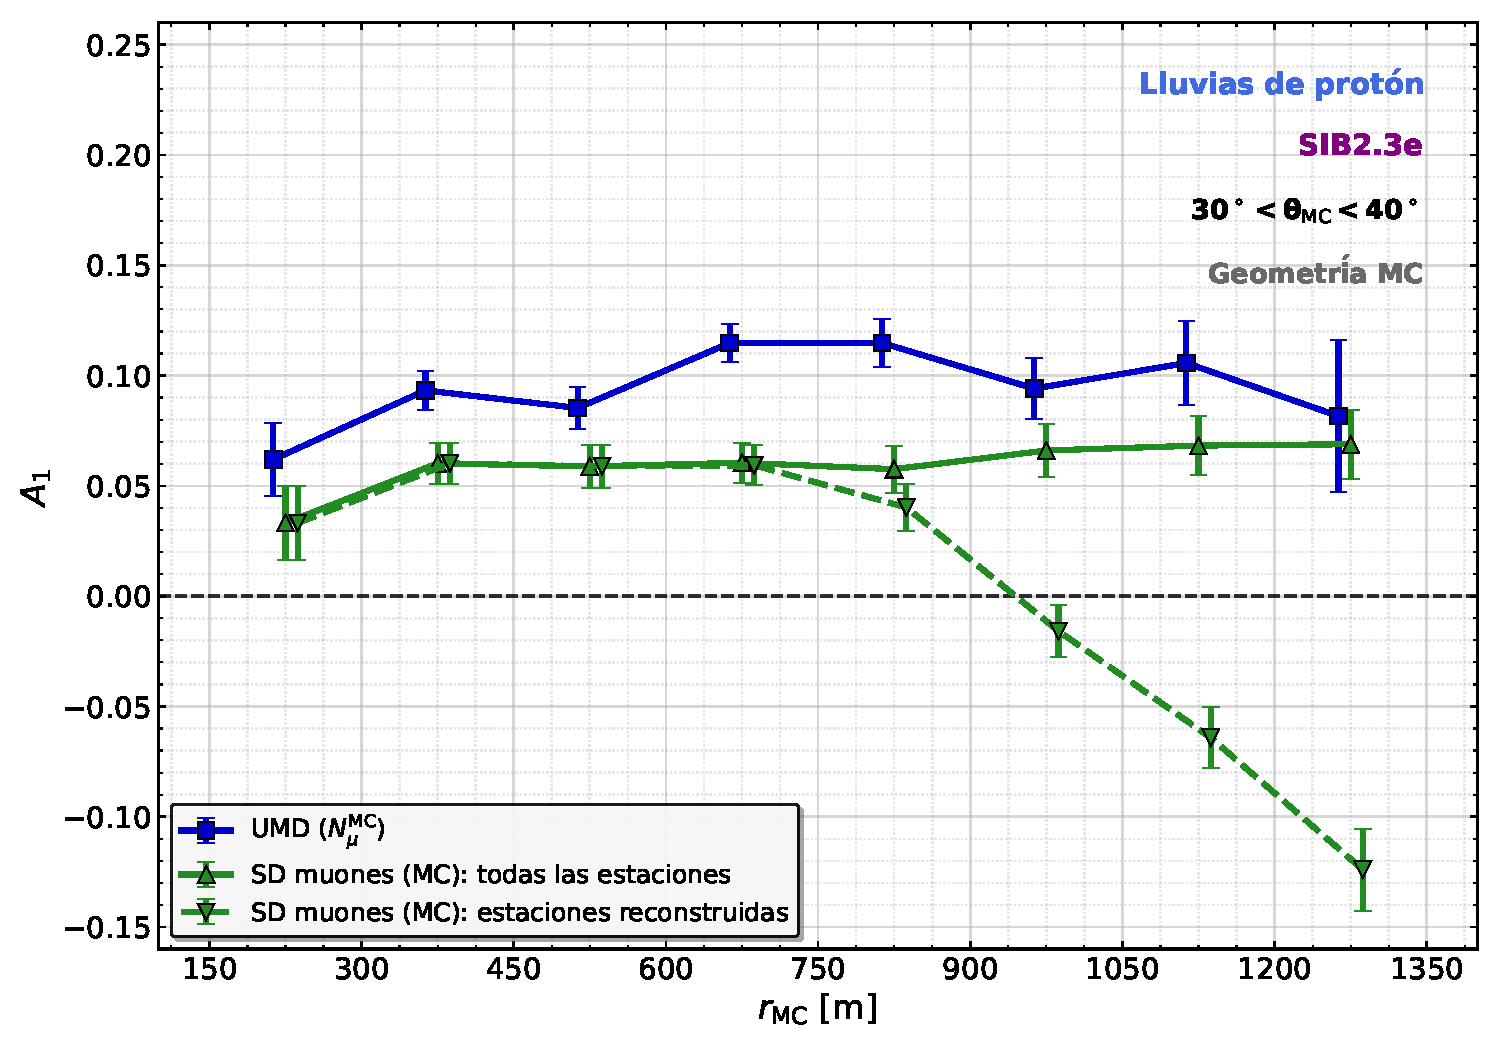
\includegraphics[width=1\textwidth]{capitulos/imagenes_capitulos/cap6/SD_Seleccion_Estaciones_vs_UMD.pdf}
	\caption{Asimetría del número de muones Monte Carlo del SD calculada sobre todas las estaciones simuladas y sólo sobre las que forman parte del evento reconstruido, junto con la del número de muones inyectado en el UMD ($N_\mu^{\mathrm{MC}}$), para $30^\circ \leq \theta < 40^\circ$ y geometría Monte Carlo. Las barras de error se obtienen con un \textit{bootstrap} sobre las lluvias de la muestra. La inversión del SD sólo aparece al restringir el promedio a las estaciones reconstruidas.}
	\label{fig:seleccion_estaciones}
\end{figure}

{\leavevmode\color{blue}El cambio de signo se obtiene con los mismos conteos, las mismas coordenadas y el mismo ajuste: lo único que cambia es qué estaciones entran en el promedio. En la banda $1200$--$1350$~m sólo el $42\%$ de las estaciones tempranas y el $18\%$ de las tardías forman parte del evento, y el cociente $\varepsilon_N/\varepsilon$ de la Ec.~\ref{eq:seleccion} vale $1.67$ y $2.28$, respectivamente: las estaciones tardías retenidas están más enriquecidas en muones que las tempranas. Una hipótesis compatible con este comportamiento es que la componente electromagnética, más intensa del lado temprano, facilita que una estación dispare aun con pocos muones, mientras que del lado tardío sólo sobreviven las estaciones con más muones. A favor de esta hipótesis, entre $900$ y $1350$~m una estación sin muones forma parte del evento en el $39\%$ de los casos en la región temprana y en el $18\%$ en la tardía, donde el número medio de partículas electromagnéticas es unas $2.4$ veces menor. Esto no prueba el mecanismo, ya que la condición de formar parte del evento resume el disparo, la lectura y la reconstrucción de la estación, y aquí no se separaron esas etapas.}

% REVISAR: chequeo nuevo de la hipótesis de selección (histograma de muones en los tanques excluidos). Figura: celda "CHEQUEO DE LA SELECCIÓN" de Scripts/plots_seccion_6.py; los números se imprimen en esa misma celda.
{\leavevmode\color{blue}Un chequeo directo de esta hipótesis consiste en contar cuántos muones atraviesan los tanques que quedan fuera de la selección. Si la inversión es un efecto de selección, las estaciones excluidas deberían ser justamente las que reciben muy pocos muones. La Figura~\ref{fig:muones_tanques_excluidos} muestra la distribución del número de muones Monte Carlo en los tanques excluidos y en los retenidos, para $900 \leq r < 1500$~m, donde conviven ambas poblaciones. Los tanques excluidos contienen como máximo un muón en el $95\%$ de los casos en la región temprana y en el $93\%$ en la tardía, con un promedio de $0.35$ y $0.46$ muones respectivamente, mientras que los retenidos tienen en promedio $1.5$ y $1.7$. Las estaciones que se pierden son, por lo tanto, las de menor contenido de muones, como exige la Ec.~\ref{eq:seleccion} para que $\varepsilon_N > \varepsilon$.}

\begin{figure}[H]
	\centering
	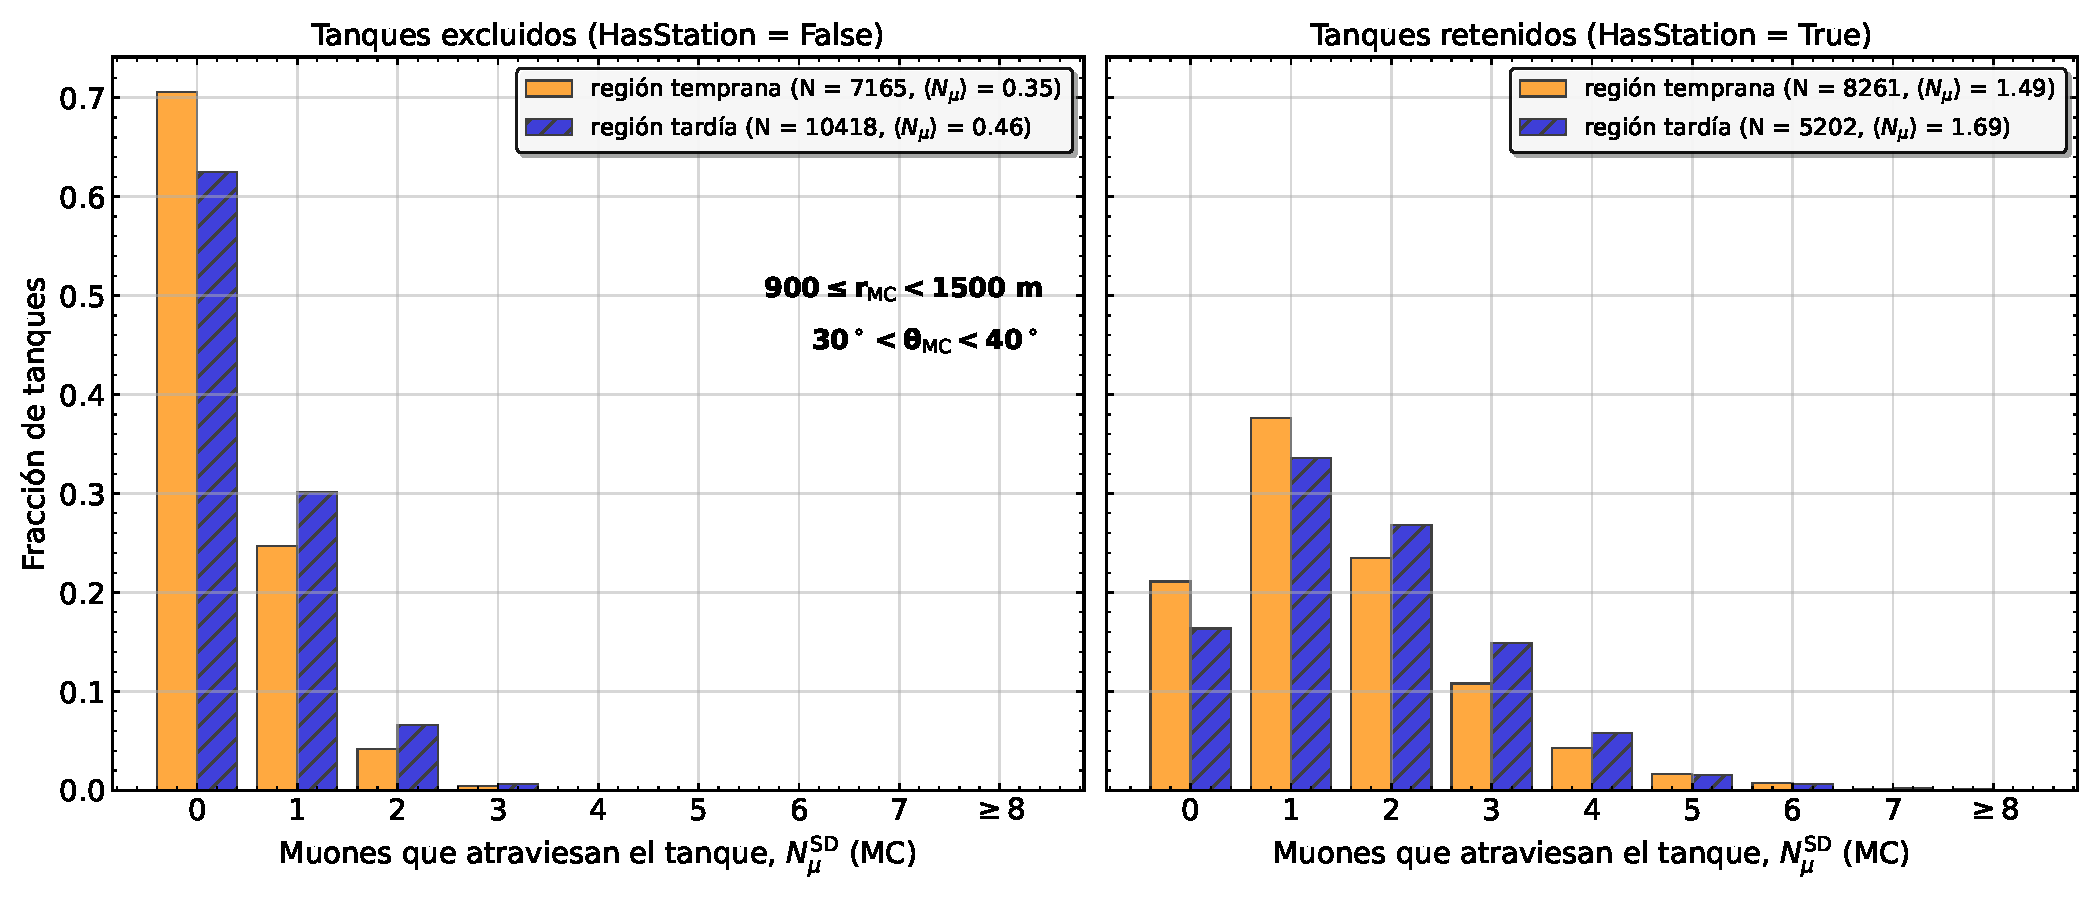
\includegraphics[width=1\textwidth]{capitulos/imagenes_capitulos/cap6/SD_Muones_Tanques_Excluidos.pdf}
	\caption{Distribución del número de muones Monte Carlo que atraviesan cada tanque del SD para las estaciones que quedan fuera del evento reconstruido (izquierda) y para las que forman parte de él (derecha), en las regiones temprana ($|\phi| < 60^\circ$) y tardía ($|\phi| > 120^\circ$). Lluvias de protón (\texttt{SIBYLL 2.3e}), $30^\circ \leq \theta < 40^\circ$, $900 \leq r < 1500$~m y geometría Monte Carlo. Cada distribución está normalizada a su número de tanques.}
	\label{fig:muones_tanques_excluidos}
\end{figure}

{\leavevmode\color{blue}La comparación entre regiones muestra además el mecanismo de la inversión. Del lado tardío se excluyen tanques con más muones que del lado temprano ($0.46$ frente a $0.35$ en promedio) pero con aproximadamente la mitad de partículas electromagnéticas ($14$ frente a $28$), es decir, del lado tardío quedan afuera estaciones que del lado temprano habrían sido retenidas gracias a su componente electromagnética. Como consecuencia, entre los tanques retenidos los tardíos terminan con más muones que los tempranos ($1.69$ frente a $1.49$), aunque la densidad de muones que llega al suelo es mayor del lado temprano. Ésta es precisamente la situación del ejemplo de Poisson de la Ec.~\ref{eq:seleccion}, y apoya la hipótesis de que la componente electromagnética determina qué estaciones se retienen.}

{\leavevmode\color{blue}Retirar el requisito tampoco hace idénticas las curvas del SD y del UMD. Entre $150$ y $900$~m, donde casi todas las estaciones son seleccionadas, el UMD presenta una asimetría entre $0.03$ y $0.06$ mayor que la de los muones del SD, una diferencia que excluye el cero al $95\%$ de confianza. Una candidata es la distinta respuesta de un detector plano y de un tanque (Sección~\ref{subsubsec:respuesta_detector}), junto con el umbral del UMD, que es más alto para las trayectorias tardías, pero esta diferencia queda abierta en este trabajo. Por otra parte, la curva del UMD también se calcula sobre los módulos de estaciones seleccionadas, y no se dispone de su conteo en las estaciones no retenidas. El efecto de la selección sobre el UMD debería ser menor, porque los muones que atraviesan los módulos enterrados no son los que hacen disparar al tanque, pero no puede descartarse a grandes distancias, donde la fracción de estaciones retenidas depende fuertemente de $\phi$.}

{\leavevmode\color{blue}En conclusión, la comparación con el UMD muestra que la asimetría de los muones medida bajo tierra se mantiene positiva a todas las distancias, mientras que la del SD se invierte por la forma en que se seleccionan las estaciones. Esto no se debe a que el blindaje filtre una población de muones blandos con asimetría negativa: según el Capítulo~\ref{sec:fenomenologia}, elevar el umbral hace a la asimetría \textit{menos} positiva. La asimetría del conteo de muones depende tanto de la respuesta del detector como de la selección de estaciones sobre la que se calcula, y la comparación entre detectores, o entre simulaciones y datos, requiere que esa selección sea la misma.}

% REVISAR: la subsección del Fast-MC queda desactivada (\iffalse ... \fi) pero intacta. Su objetivo declarado ("probar [...] que la asimetría negativa es un artefacto geométrico exclusivo de la Población B y que el UMD lo anula") quedó refutado por el Cap. 3 y por el control de selección. Los pasos 1-3 siguen siendo una buena forma de predecir AMPLITUDES (el modelo de juguete del Cap. 3 no lo hace). Sugerencia para el Cap. 8 (Perspectivas):
% "Una extensión natural de este trabajo es predecir cuantitativamente la amplitud $A_1$ a partir de la cinemática de producción, extrayendo de simulaciones dedicadas de CORSIKA las distribuciones $F(X,E_i,p_t)$, propagando los muones con el modelo de Cazón \textit{et al.} \cite{Cazon2012} y proyectándolos sobre el suelo con la respuesta y el umbral de cada detector, en lugar de la fuente puntual del modelo de juguete del Capítulo~\ref{sec:fenomenologia}."
\iffalse
\subsection{Propuesta de Modelado del Filtro Cinemático}
\label{subsec:fast_mc}

Si bien el análisis de las simulaciones procesadas con el \textit{framework Offline} ha demostrado de manera contundente la degradación sistemática de la asimetría azimutal en el Detector de Superficie (SD) y su preservación en el Detector Subterráneo de Muones (UMD), la demostración del mecanismo propuesto en la sección anterior para explicar la competencia entre efectos y la diferencia fenomenológica entre detectores requiere un abordaje desde primeros principios. 

La limitación intrínseca de este estudio radica en que las simulaciones utilizadas entregan la huella final de la lluvia a nivel del suelo, careciendo de la granularidad necesaria para rastrear la cinemática de producción individual ($p_z$, $p_t$ y altura de decaimiento $z$) de cada partícula antes de su propagación. Para probar de manera aislada que la asimetría negativa es un artefacto geométrico exclusivo de la Población B y que el UMD lo anula por completo, se deja planteado como perspectiva a futuro, excediendo los alcances del presente trabajo, el desarrollo de un \textit{Toy Model} fenomenológico (un propagador \textit{Fast-Monte Carlo}).

La hoja de ruta propuesta para implementar este modelo en futuras investigaciones, el cual acoplaría la producción hadrónica con el transporte analítico de los muones, se estructuraría en las siguientes etapas:

\begin{enumerate}
	\item \textbf{Extracción de las distribuciones de producción:} Generar un lote de simulaciones dedicadas en CORSIKA con el único fin de extraer la función de distribución tridimensional en el punto de decaimiento del hadrón progenitor: $F(X, E_i, p_t)$. De esta forma, se obtiene el espectro de energía inicial y momento transversal real en función de la profundidad atmosférica $X$.
	
	\item \textbf{Propagación analítica y supervivencia:} A partir de $F(X, E_i, p_t)$, aplicar técnicas de remuestreo (\textit{Bootstrap} o Monte Carlo) para inyectar muones y propagarlos analíticamente hacia el suelo. Esta etapa utilizará el modelo de transporte cinemático de L. Cazón \textit{et al.} \cite{Cazon2012}, aplicando la isoterma atmosférica para calcular las pérdidas continuas de energía por ionización ($dE/dX$) y evaluar la probabilidad de supervivencia frente al decaimiento en vuelo.
	
	\item \textbf{Proyección geométrica e impacto:} Intersecar las trayectorias resultantes con el plano inclinado del arreglo de superficie. Este paso introducirá de forma natural la excentricidad geométrica, permitiendo evaluar cómo la divergencia radial de cada partícula afecta su fase azimutal de impacto.
	
	\item \textbf{El filtro instrumental:} Al obtener la energía final residual a nivel del suelo ($E_f$), se aplicarán funciones escalón para emular los diferentes umbrales instrumentales. Se evaluará la densidad total (emulando la respuesta muónica del SD) y se contrastará contra la distribución aplicando un umbral cinemático estricto de $E_f \gtrsim 1.0\text{ GeV}$ (emulando el blindaje pasivo del UMD).
\end{enumerate}

Una vez concretado en trabajos posteriores, este marco permitirá demostrar de forma completamente analítica cómo el espectro de baja energía, al poseer ángulos de divergencia masivos, dispara el término geométrico $\langle p_r / -p_z \rangle$ forzando la asimetría negativa ($A_1 < 0$) en el \textit{far-core}. Simultáneamente, probará desde las ecuaciones fundamentales de transporte que la barrera de atenuación del UMD filtra las trayectorias de bajo momento longitudinal, anulando la distorsión proyectiva de manera determinista y revelando únicamente la asimetría positiva intrínseca al desarrollo longitudinal de la lluvia.
\fi

\section{Arreglo \textit{Infill} usando la geometría reconstruida}
\label{subsec:infill_rec}

% REVISAR: verificá la definición exacta de la "geometría REC". Según Procesamiento_ADST_v8-2.py (l. 302-330), r_core es la distancia al núcleo reconstruido calculada con los ángulos MC, phi_REC sale de GetAzimuthSP, y en plots_seccion_6.py las bandas de theta son en theta_MC también en modo REC. El Cap. 7 usa theta_REC.
Habiendo caracterizado la fenomenología pura de la cascada utilizando el escenario ideal (núcleo y ángulos Monte Carlo), el análisis se traslada en el contexto de simulaciones al entorno experimental más realista posible. En esta sección, el cálculo de las coordenadas y fases azimutales en el plano de la lluvia se realiza utilizando la posición del centro de impacto y los ángulos de arribo reportados por el algoritmo de reconstrucción del Observatorio (geometría \textit{REC}).

Al igual que en el estudio con geometría ideal, la transición de utilizar la cantidad de muones inyectados ($N_\mu^{\mathrm{MC}}$) a la de muones reconstruidos por la electrónica del UMD ($N_\mu^{\mathrm{REC}}$) conserva la forma de la evolución de la asimetría, solo afectando débilmente su magnitud debido a los sesgos direccionales del algoritmo. Sin embargo, al introducir la incertidumbre espacial de la \textbf{geometría reconstruida}, el panorama fenomenológico cambia drásticamente para todos los detectores: la modulación azimutal se ve severamente comprometida, perdiéndose la capacidad de detectar asimetría en diversas regiones radiales.

El análisis sistemático de los ajustes armónicos sobre los datos reconstruidos permite mapear de manera transparente los límites resolutivos y estadísticos del arreglo \textit{Infill} al menos en el marco de simulaciones:

\begin{itemize}
	\item \textbf{Régimen cuasi-vertical ($0^\circ \le \theta < 20^\circ$):} La asimetría es físicamente marginal y la reconstrucción apenas logra identificar modulaciones débiles en un rango acotado ($450 \le r \le 1050\text{ m}$). Fuera de esta ventana, las fluctuaciones dominan sobre el gradiente direccional.
	
	\item \textbf{Régimen de transición ($20^\circ \le \theta < 40^\circ$):} Se establece una clara ventana de máxima fidelidad fenomenológica entre los $650\text{ m}$ y los $1200\text{ m}$. Los ajustes armónicos convergen con valores de $\chi^2/\mathrm{ndf}$ estables y barras de error acotadas pero la magnitud de la asimetría es baja y no sigue el comportamiento esperado de aumentar a medida que el bin radial aumenta {\color{blue}(ver Sección~\ref{subsec:lavado_nucleo})}. Para distancias superiores ($r > 1200\text{ m}$), la densidad muónica decae drásticamente.

	% REVISAR: faltaba la banda 40-50 grados, que es la de referencia de la Figura fig:umd_rec_vs_mc_theta y la que usa el Cap. 7. Los valores son aproximados (con N_mu^MC y theta_MC, referencia_intento_descartado/descomposicion_geometria_REC.csv): -0.03 a 300 m, ~0 a 450 m y 0.03-0.05 entre 600 y 1050 m. Confirmalos con tu grilla del Anexo (fig:anexo_grilla_rec_40_50), que usa N_mu^REC.
	\item \textbf{Régimen inclinado ($40^\circ \le \theta < 50^\circ$):} {\color{blue}Con la geometría reconstruida la asimetría resulta positiva pero pequeña ($A_1 \lesssim 0.05$) entre $600$ y $1050$~m, frente a $A_1 \approx 0.11$ con la geometría Monte Carlo, y se anula o se vuelve levemente negativa por debajo de $450$~m. Es la banda con mayor corrimiento del núcleo reconstruido (Sección~\ref{subsec:lavado_nucleo}).}

	% REVISAR: "inmensa" -> "gran".
	\item \textbf{Régimen de alta inclinación ($50^\circ \le \theta < 65^\circ$):} Debido a la gran proyección del disco muónico sobre el suelo para lluvias rasantes, la estadística de conteo se mantiene elevada a grandes distancias. Esto permite que el ajuste armónico sobreviva con notable estabilidad y magnitud desde los $600\text{ m}$ hasta la periferia más lejana del arreglo ($1500\text{ m}$), consolidando a este rango como el escenario óptimo para el estudio de asimetrías de atenuación en el \textit{far-core}.
\end{itemize}

% REVISAR: se reemplaza la explicación por "smearing angular". Recalculando la asimetría con cada coordenada por separado, usar el azimut reconstruido no cambia A1 (< 0.01); toda la pérdida viene de la distancia al núcleo reconstruido, que está corrido de forma sistemática hacia la región temprana (Cap. 5, subsubsec:corrimiento_nucleo). Esto es lo que el Cap. 5 (l. 147 del DRAFT) promete que se muestra acá.
% ORIGINAL: "Este fenómeno de degradación responde a una difusión o \textit{smearing} angular. La incertidumbre espacial intrínseca en la determinación del núcleo del arreglo \textit{Infill} ($\sigma_{core} \approx 20 - 40$~m) propaga un error continuo en el cálculo del azimut asignado a cada estación ($\Delta \phi$). [...] actuando como un filtro pasa-bajos espacial que "plancha" la modulación cosenoidal. El efecto es especialmente destructivo cerca del núcleo ($r \lesssim 400$~m), donde un leve corrimiento del centro de impacto invierte por completo el vector de posición, justificando la necesidad estricta del corte fiducial aplicado."
\subsection{Origen de la degradación: el corrimiento del núcleo}
\label{subsec:lavado_nucleo}

{\leavevmode\color{blue}Este fenómeno de degradación no responde a una difusión aleatoria del azimut asignado a cada estación, sino al corrimiento sistemático del núcleo reconstruido hacia la región temprana descripto en la Sección~\ref{subsubsec:corrimiento_nucleo} (Figura~\ref{fig:bias_core_azimut}), de $b \simeq 9$, $15$ y $21$~m para $\theta$ entre $20^\circ$--$30^\circ$, $30^\circ$--$40^\circ$ y $40^\circ$--$50^\circ$. Con la geometría reconstruida, las estaciones tempranas se ubican más cerca del núcleo de lo que realmente están y las tardías más lejos. Dentro de un mismo bin radial, las estaciones tempranas provienen entonces de distancias verdaderas mayores, con menos muones, y las tardías de distancias menores, con más. Si la densidad decae localmente como $\rho \propto r^{-\beta}$, la amplitud medida con la geometría reconstruida se reduce en
\begin{equation}
	\Delta A_1 \simeq -\beta\,\frac{b}{r},
	\label{eq:lavado_nucleo}
\end{equation}
un efecto que crece hacia el núcleo y con la inclinación de la lluvia, y que en las lluvias inclinadas puede volver negativa la asimetría a distancias cortas.}

{\leavevmode\color{blue}Para verificarlo, se recalculó la asimetría del UMD sobre los mismos módulos y con el número de muones inyectado, reemplazando por separado la distancia y el azimut verdaderos por los reconstruidos. La Tabla~\ref{tab:lavado_nucleo} resume el resultado para el bin $450 \leq r < 600$~m. Reemplazar el azimut prácticamente no modifica la asimetría, mientras que reemplazar la distancia la reduce casi por completo, y la reducción coincide con la predicción de la Ec.~\ref{eq:lavado_nucleo}, calculada con el corrimiento $b$ del Capítulo~\ref{sec:cap_anillo_denso} y la pendiente local $\beta$ de la LDF de los mismos módulos.}

% REVISAR: tabla nueva. Fuente: claude_work/capitulo6_infill_2026_10_07/referencia_intento_descartado/descomposicion_geometria_REC.csv (+ Cap6_infill.py, sección 9). Protones, N_mu^MC, theta_MC, sólo eventos reconstruidos; errores por bootstrap sobre lluvias (~0.007-0.011 por valor). Entre 300 y 1350 m la diferencia entre lo observado y lo predicho es menor que 0.03 en todas las celdas salvo dos. Si preferís una figura en lugar de la tabla, se agrega como celda en plots_seccion_6.py.
\begin{table}[H]
	\centering
	\begin{tabular}{lccccccc}
		\toprule
		$\theta$ & $(r_{MC},\phi_{MC})$ & $(r_{MC},\phi_{REC})$ & $(r_{REC},\phi_{MC})$ & $(r_{REC},\phi_{REC})$ & $\beta$ & $\Delta A_1$ obs. & $-\beta b/r$ \\
		\midrule
		$20^\circ$--$30^\circ$ & $0.062$ & $0.061$ & $0.011$ & $0.011$ & $2.9$ & $-0.051$ & $-0.051$ \\
		$30^\circ$--$40^\circ$ & $0.086$ & $0.084$ & $0.002$ & $0.002$ & $2.7$ & $-0.084$ & $-0.081$ \\
		$40^\circ$--$50^\circ$ & $0.108$ & $0.107$ & $-0.001$ & $-0.002$ & $2.5$ & $-0.110$ & $-0.102$ \\
		\bottomrule
	\end{tabular}
	\caption{Asimetría $A_1$ del número de muones inyectado en el UMD para $450 \leq r < 600$~m, calculada con la distancia y el azimut respecto del núcleo verdadero (MC) o reconstruido (REC). $\Delta A_1$ es la diferencia entre la geometría reconstruida y la verdadera, y la última columna es la predicción de la Ec.~\ref{eq:lavado_nucleo}. Los errores estadísticos de cada valor son de $\sim 0.01$.}
	\label{tab:lavado_nucleo}
\end{table}

{\leavevmode\color{blue}El lavado de la asimetría proviene, por lo tanto, de la distancia asignada a cada estación y no de su azimut: un corrimiento de $\sim 15$~m desplaza el azimut de una estación a $450$~m en apenas $\sim 2^\circ$, mucho menos que el ancho de los bines de $30^\circ$. Este efecto no se presenta en el Anillo Denso, cuyas estaciones se ubican a $450$~m del núcleo verdadero (Sección~\ref{subsubsec:corrimiento_nucleo}), y explica por qué la geometría reconstruida borra la modulación en el \textit{Infill}.}



\subsection{Resiliencia de la componente electromagnética en la reconstrucción}
\label{subsec:em_rec}

Al repetir el análisis de competencia entre el UMD y el SD, pero ahora sujetos a la degradación geométrica de la reconstrucción, emerge una conclusión inesperada al desglosar la señal del tanque Cherenkov.

% REVISAR: "smearing angular" -> "corrimiento del núcleo".
{\color{blue}A pesar de que el corrimiento del núcleo} destruye gran parte de la modulación en la componente muónica del UMD y del SD, el ajuste armónico sobre la componente electromagnética (SD EM) revela que esta preserva una asimetría fuertemente positiva y altamente significativa a lo largo de todos los bines radiales evaluados. Aún bajo los efectos de la incertidumbre topográfica, la señal EM se ajusta con barras de error estadístico notablemente pequeñas.

% REVISAR: la abundancia de partículas achica las barras de error, pero no protege de un corrimiento sistemático. Lo que mantiene positiva a la EM es que su asimetría es mucho mayor que el término -beta*b/r. Números: referencia_intento_descartado/descomposicion_SD_30_40.csv.
% ORIGINAL: "Esta excepcional resiliencia no implica que los fotones y electrones sean inmunes al error de reconstrucción, sino que es una consecuencia directa de su abrumadora abundancia estadística. [...] La asimetría física generada por este vaciamiento atmosférico es tan profunda y estadísticamente rica que logra sobreponerse a la "borrosidad" espacial introducida por el desplazamiento del núcleo."
{\color{blue}Esta resiliencia no implica que los fotones y electrones sean inmunes al error de reconstrucción. El corrimiento del núcleo reduce la asimetría electromagnética en una cantidad similar a la muónica, de $0.41$ a $0.31$ en el bin $450$--$600$~m para $30^\circ \leq \theta < 40^\circ$, pero como su asimetría es varias veces mayor, sigue siendo claramente positiva. La abundancia estadística de la componente electromagnética reduce las barras de error, pero no la protege frente a un corrimiento sistemático.}

% REVISAR: título y segundo párrafo nuevos. El original explicaba la persistencia con los muones blandos y A_geo que "explota", lo que contradice el Cap. 3. Números: referencia_intento_descartado/descomposicion_SD_30_40.csv.
% ORIGINAL título: "La supervivencia de la asimetría geométrica muónica".
% ORIGINAL (resumen): "Como se desarrolló en la sección analítica, la asimetría negativa es impulsada por la población de muones blandos [...] el término de asimetría geométrica de Billoir [...] explota a grandes distancias radiales. [...] confirmando que este artefacto no es una falla de Monte Carlo, sino un obstáculo experimental empírico."
{\color{blue}\subsection{La inversión del SD con la geometría reconstruida}
\label{subsec:inversion_sd_rec}}

Por el contrario, la inversión de la asimetría del observable total del SD hacia valores negativos en el \textit{far-core} se sigue manifestando en los datos reconstruidos. Esta inversión encuentra su justificación en la naturaleza de la parte muónica del SD.

{\color{blue}Como la selección de estaciones no depende de la geometría asignada, el efecto descripto en la Sección~\ref{subsec:seleccion_estaciones} se mantiene, mientras que el corrimiento del núcleo, proporcional a $b/r$, es pequeño a grandes distancias: en el bin $1200$--$1350$~m la asimetría de los muones del SD vale $-0.125$ con la geometría Monte Carlo y $-0.132$ con la reconstruida. La inversión es, por lo tanto, una propiedad del observable y de la muestra de estaciones sobre la que se calcula, y debe esperarse también en los datos de campo, que se seleccionan de la misma manera.}

\section{Comparación de performance: UMD Monte Carlo vs. UMD Reconstruido}
\label{subsec:comparacion_performance_umd}

Habiendo justificado el comportamiento del SD, el foco recae finalmente sobre la performance del Detector Subterráneo de Muones frente a las incertezas de la reconstrucción. Al comparar directamente los ajustes obtenidos para el UMD utilizando la geometría Monte Carlo contra aquellos obtenidos con la geometría Reconstruida, se consolida una métrica del poder resolutivo del instrumento.

% REVISAR: se reemplaza el párrafo borrador. "Filtrar cinemáticamente a la población blanda" contradice el Cap. 3, y la geometría REC no da una "cota inferior": le resta a A1 un término calculable (Ec. eq:lavado_nucleo), no la escala.
% ORIGINAL: "La comparativa evidencia que, si bien el UMD logra filtrar cinemáticamente a la población blanda y aislar la asimetría positiva en el mundo ideal, la introducción de los errores de reconstrucción del arreglo de superficie (Core REC) impone una cota experimental a la amplitud observable. La difusión angular "achata" las curvas de $A_1$, indicando que las asimetrías medidas experimentalmente representarán sistemáticamente un límite inferior (\textit{lower bound}) de la verdadera polaridad de la cascada. Maximizar la precisión algorítmica en la ubicación del núcleo resulta, por lo tanto, tan determinante para medir la atenuación como lo es el propio blindaje del detector."
{\leavevmode\color{blue}La diferencia entre $A_1^{\mathrm{REC}}$ y $A_1^{\mathrm{MC}}$ en el UMD puede separarse en tres contribuciones. La primera es la reconstrucción del número de muones, que con la geometría fija reduce la asimetría entre un $5$ y un $23\%$ sin cambiar su forma (Figura~\ref{fig:umd_rec_vs_mc_theta}), por el sesgo direccional del algoritmo (Sección~\ref{subsec:bias_direccional}). La segunda es el azimut reconstruido, cuyo efecto es despreciable. La tercera, y dominante, es la distancia al núcleo reconstruido, que resta a la asimetría el término de la Ec.~\ref{eq:lavado_nucleo} (Tabla~\ref{tab:lavado_nucleo}).}

{\leavevmode\color{blue}La comparativa evidencia, por lo tanto, que la geometría reconstruida reduce de manera sistemática la amplitud observable. Esta reducción no es una pérdida aleatoria de resolución, sino un corrimiento que puede estimarse a partir de $b$ y de la pendiente de la LDF, y que por lo tanto podría corregirse o incluirse en la comparación con los datos. La ventana en la que la asimetría reconstruida se mantiene positiva y medible, $600 \leq r < 1200$~m y $20^\circ \leq \theta < 55^\circ$, es la región de referencia utilizada en el Capítulo~\ref{sec:datos_reales}. Mejorar la determinación del núcleo, por ejemplo con un ajuste de la LDF que incluya la modulación azimutal, resulta tan determinante para medir la asimetría como la propia respuesta del detector.}

% REVISAR: sección nueva, armada a partir de tus notas ("VER SI PUEDO AGREGAR A A1(R, THETA) UNA DEPENDENCIA CON PRIMARIO Y ENERGIA [...] TODO ESTO LO HARIA EN UNA SECCION APARTE Y LAS SUBSECCIONES SERIAN VER QUE PASA CON LA PARTE USANDO COSAS MC Y CON LA REC").
% Números: claude_work/capitulo6_infill_2026_10_07/referencia_intento_descartado/ (resumen_Fe_menos_p.csv, diferencia_Fe_menos_p.csv, resumen_subbandas_energia.csv; código en Cap6_infill.py, secciones 10-11). Estimador: el mismo ajuste, con errores por bootstrap sobre lluvias; en geometría REC las bandas son en theta_REC, como en el Cap. 7.
% No hay figura todavía: si la querés, la agrego como celda de plots_seccion_6.py en tu estilo.
\section{Dependencia con el primario y la energía}
\label{sec:infill_masa}

{\leavevmode\color{blue}Habiendo caracterizado la asimetría para lluvias de protón, se evaluó si el arreglo \textit{Infill} conserva la sensibilidad a la masa del primario observada en el Anillo Denso (Sección~\ref{sec:discriminacion_masa}). Para esto se repitió el análisis con las bibliotecas de helio y hierro (\texttt{SIBYLL 2.3e}, mismo rango de energía) en las dos franjas cenitales de mayor discriminación en el Anillo Denso, $30^\circ \leq \theta < 40^\circ$ y $40^\circ \leq \theta < 50^\circ$, primero con la geometría Monte Carlo y luego con la reconstruida.}

\subsection{Geometría Monte Carlo}

{\leavevmode\color{blue}Con la geometría Monte Carlo, la asimetría del hierro resulta levemente menor que la del protón en casi todos los bines radiales entre $300$ y $1050$~m, en el mismo sentido que en el Anillo Denso. Sin embargo, la diferencia en cada bin es del orden de su incertidumbre ($\sim 0.01$--$0.03$). Promediando los diez bines entre $450$ y $1200$~m de ambas franjas, con pesos iguales a la inversa de su varianza, se obtiene $\langle A_1^{\mathrm{Fe}} - A_1^{\mathrm{p}} \rangle = -0.010 \pm 0.005$, una separación de $\sim 2\sigma$. El helio se ubica entre ambos o se superpone con ellos dentro de los errores. A diferencia del Anillo Denso, donde las doce estaciones virtuales se ubican siempre a la misma distancia del núcleo, cada bin del \textit{Infill} contiene pocas estaciones por lluvia, y la incertidumbre resultante es comparable a la diferencia esperada entre primarios.}

\subsection{Geometría reconstruida}

{\leavevmode\color{blue}Con la geometría reconstruida la separación desaparece: $\langle A_1^{\mathrm{Fe}} - A_1^{\mathrm{p}} \rangle = -0.003 \pm 0.005$, compatible con cero, en acuerdo con lo encontrado en el Capítulo~\ref{sec:datos_reales}. El corrimiento del núcleo resta a ambos primarios un término de magnitud similar o mayor que la diferencia buscada, y como ese corrimiento depende del propio desarrollo de la lluvia, podría además diferir entre primarios. En el arreglo \textit{Infill}, y con la estadística simulada, la asimetría reconstruida del UMD no permite por lo tanto discriminar entre protón y hierro.}

\subsection{Dependencia con la energía}

% REVISAR: tu nota planteaba 5 bines de energía como en el Anillo Denso; en el Infill eso deja muy poca estadística por celda, así que se usan dos sub-bandas.
{\leavevmode\color{blue}Un bineado en cinco intervalos de energía, como el utilizado en el Anillo Denso (Sección~\ref{subsec:dependencia_energia}), deja muy pocas estaciones por celda en el \textit{Infill}. Dividiendo el rango simulado en dos sub-bandas y promediando los mismos diez bines con la geometría Monte Carlo, la asimetría del protón pasa de $0.110 \pm 0.005$ en $17.50 \leq \log_{10}(E/\mathrm{eV}) < 17.75$ a $0.118 \pm 0.004$ en $17.75$--$18.00$, y la del hierro de $0.102 \pm 0.004$ a $0.105 \pm 0.003$. Ambas variaciones tienen el signo y el orden de magnitud del crecimiento observado en el Anillo Denso, pero no son significativas. Un estudio de la dependencia con la energía en el \textit{Infill} requiere bibliotecas de simulaciones que cubran un rango más amplio.}

% REVISAR: tu nota sobre el ángulo de incidencia ("PODRIA VER [...] O MERAMENTE DECLARARLO"): se declara en una oración, remitiendo al Anillo Denso.
{\leavevmode\color{blue}Por último, no se estudió la dependencia con el azimut de arribo de la lluvia en el \textit{Infill}: en el Anillo Denso la asimetría resultó independiente de él (Sección~\ref{subsubsec:invariancia_phi}), y la estadística disponible en el \textit{Infill} no permitiría resolver variaciones de ese orden.}

% REVISAR: se eliminaron las notas en mayúsculas del final (DESPUES PASAMOS A HABLAR DE LO MISMO [...] PUEDE SER QUE DE MEDIO RARO). Los puntos 1-3 y 5 ya estaban cubiertos por tu prosa de la geometría REC y por la nueva subsección de selección de estaciones; los puntos 4, 6 y 7 son las dos secciones de arriba.

\newpage
